% Options for packages loaded elsewhere
\PassOptionsToPackage{unicode}{hyperref}
\PassOptionsToPackage{hyphens}{url}
\PassOptionsToPackage{dvipsnames,svgnames,x11names}{xcolor}
%
\documentclass[
]{article}

\usepackage{amsmath,amssymb}
\usepackage{iftex}
\ifPDFTeX
  \usepackage[T1]{fontenc}
  \usepackage[utf8]{inputenc}
  \usepackage{textcomp} % provide euro and other symbols
\else % if luatex or xetex
  \usepackage{unicode-math}
  \defaultfontfeatures{Scale=MatchLowercase}
  \defaultfontfeatures[\rmfamily]{Ligatures=TeX,Scale=1}
\fi
\usepackage{lmodern}
\ifPDFTeX\else  
    % xetex/luatex font selection
\fi
% Use upquote if available, for straight quotes in verbatim environments
\IfFileExists{upquote.sty}{\usepackage{upquote}}{}
\IfFileExists{microtype.sty}{% use microtype if available
  \usepackage[]{microtype}
  \UseMicrotypeSet[protrusion]{basicmath} % disable protrusion for tt fonts
}{}
\makeatletter
\@ifundefined{KOMAClassName}{% if non-KOMA class
  \IfFileExists{parskip.sty}{%
    \usepackage{parskip}
  }{% else
    \setlength{\parindent}{0pt}
    \setlength{\parskip}{6pt plus 2pt minus 1pt}}
}{% if KOMA class
  \KOMAoptions{parskip=half}}
\makeatother
\usepackage{xcolor}
\setlength{\emergencystretch}{3em} % prevent overfull lines
\setcounter{secnumdepth}{-\maxdimen} % remove section numbering
% Make \paragraph and \subparagraph free-standing
\makeatletter
\ifx\paragraph\undefined\else
  \let\oldparagraph\paragraph
  \renewcommand{\paragraph}{
    \@ifstar
      \xxxParagraphStar
      \xxxParagraphNoStar
  }
  \newcommand{\xxxParagraphStar}[1]{\oldparagraph*{#1}\mbox{}}
  \newcommand{\xxxParagraphNoStar}[1]{\oldparagraph{#1}\mbox{}}
\fi
\ifx\subparagraph\undefined\else
  \let\oldsubparagraph\subparagraph
  \renewcommand{\subparagraph}{
    \@ifstar
      \xxxSubParagraphStar
      \xxxSubParagraphNoStar
  }
  \newcommand{\xxxSubParagraphStar}[1]{\oldsubparagraph*{#1}\mbox{}}
  \newcommand{\xxxSubParagraphNoStar}[1]{\oldsubparagraph{#1}\mbox{}}
\fi
\makeatother

\usepackage{color}
\usepackage{fancyvrb}
\newcommand{\VerbBar}{|}
\newcommand{\VERB}{\Verb[commandchars=\\\{\}]}
\DefineVerbatimEnvironment{Highlighting}{Verbatim}{commandchars=\\\{\}}
% Add ',fontsize=\small' for more characters per line
\newenvironment{Shaded}{}{}
\newcommand{\AlertTok}[1]{\textcolor[rgb]{1.00,0.00,0.00}{\textbf{#1}}}
\newcommand{\AnnotationTok}[1]{\textcolor[rgb]{0.38,0.63,0.69}{\textbf{\textit{#1}}}}
\newcommand{\AttributeTok}[1]{\textcolor[rgb]{0.49,0.56,0.16}{#1}}
\newcommand{\BaseNTok}[1]{\textcolor[rgb]{0.25,0.63,0.44}{#1}}
\newcommand{\BuiltInTok}[1]{\textcolor[rgb]{0.00,0.50,0.00}{#1}}
\newcommand{\CharTok}[1]{\textcolor[rgb]{0.25,0.44,0.63}{#1}}
\newcommand{\CommentTok}[1]{\textcolor[rgb]{0.38,0.63,0.69}{\textit{#1}}}
\newcommand{\CommentVarTok}[1]{\textcolor[rgb]{0.38,0.63,0.69}{\textbf{\textit{#1}}}}
\newcommand{\ConstantTok}[1]{\textcolor[rgb]{0.53,0.00,0.00}{#1}}
\newcommand{\ControlFlowTok}[1]{\textcolor[rgb]{0.00,0.44,0.13}{\textbf{#1}}}
\newcommand{\DataTypeTok}[1]{\textcolor[rgb]{0.56,0.13,0.00}{#1}}
\newcommand{\DecValTok}[1]{\textcolor[rgb]{0.25,0.63,0.44}{#1}}
\newcommand{\DocumentationTok}[1]{\textcolor[rgb]{0.73,0.13,0.13}{\textit{#1}}}
\newcommand{\ErrorTok}[1]{\textcolor[rgb]{1.00,0.00,0.00}{\textbf{#1}}}
\newcommand{\ExtensionTok}[1]{#1}
\newcommand{\FloatTok}[1]{\textcolor[rgb]{0.25,0.63,0.44}{#1}}
\newcommand{\FunctionTok}[1]{\textcolor[rgb]{0.02,0.16,0.49}{#1}}
\newcommand{\ImportTok}[1]{\textcolor[rgb]{0.00,0.50,0.00}{\textbf{#1}}}
\newcommand{\InformationTok}[1]{\textcolor[rgb]{0.38,0.63,0.69}{\textbf{\textit{#1}}}}
\newcommand{\KeywordTok}[1]{\textcolor[rgb]{0.00,0.44,0.13}{\textbf{#1}}}
\newcommand{\NormalTok}[1]{#1}
\newcommand{\OperatorTok}[1]{\textcolor[rgb]{0.40,0.40,0.40}{#1}}
\newcommand{\OtherTok}[1]{\textcolor[rgb]{0.00,0.44,0.13}{#1}}
\newcommand{\PreprocessorTok}[1]{\textcolor[rgb]{0.74,0.48,0.00}{#1}}
\newcommand{\RegionMarkerTok}[1]{#1}
\newcommand{\SpecialCharTok}[1]{\textcolor[rgb]{0.25,0.44,0.63}{#1}}
\newcommand{\SpecialStringTok}[1]{\textcolor[rgb]{0.73,0.40,0.53}{#1}}
\newcommand{\StringTok}[1]{\textcolor[rgb]{0.25,0.44,0.63}{#1}}
\newcommand{\VariableTok}[1]{\textcolor[rgb]{0.10,0.09,0.49}{#1}}
\newcommand{\VerbatimStringTok}[1]{\textcolor[rgb]{0.25,0.44,0.63}{#1}}
\newcommand{\WarningTok}[1]{\textcolor[rgb]{0.38,0.63,0.69}{\textbf{\textit{#1}}}}

\providecommand{\tightlist}{%
  \setlength{\itemsep}{0pt}\setlength{\parskip}{0pt}}\usepackage{longtable,booktabs,array}
\usepackage{calc} % for calculating minipage widths
% Correct order of tables after \paragraph or \subparagraph
\usepackage{etoolbox}
\makeatletter
\patchcmd\longtable{\par}{\if@noskipsec\mbox{}\fi\par}{}{}
\makeatother
% Allow footnotes in longtable head/foot
\IfFileExists{footnotehyper.sty}{\usepackage{footnotehyper}}{\usepackage{footnote}}
\makesavenoteenv{longtable}
\usepackage{graphicx}
\makeatletter
\newsavebox\pandoc@box
\newcommand*\pandocbounded[1]{% scales image to fit in text height/width
  \sbox\pandoc@box{#1}%
  \Gscale@div\@tempa{\textheight}{\dimexpr\ht\pandoc@box+\dp\pandoc@box\relax}%
  \Gscale@div\@tempb{\linewidth}{\wd\pandoc@box}%
  \ifdim\@tempb\p@<\@tempa\p@\let\@tempa\@tempb\fi% select the smaller of both
  \ifdim\@tempa\p@<\p@\scalebox{\@tempa}{\usebox\pandoc@box}%
  \else\usebox{\pandoc@box}%
  \fi%
}
% Set default figure placement to htbp
\def\fps@figure{htbp}
\makeatother

\usepackage{fvextra}
\DefineVerbatimEnvironment{Highlighting}{Verbatim}{breaklines=true,breakanywhere=true,commandchars=\\\{\}}
\makeatletter
\@ifpackageloaded{caption}{}{\usepackage{caption}}
\AtBeginDocument{%
\ifdefined\contentsname
  \renewcommand*\contentsname{Table of contents}
\else
  \newcommand\contentsname{Table of contents}
\fi
\ifdefined\listfigurename
  \renewcommand*\listfigurename{List of Figures}
\else
  \newcommand\listfigurename{List of Figures}
\fi
\ifdefined\listtablename
  \renewcommand*\listtablename{List of Tables}
\else
  \newcommand\listtablename{List of Tables}
\fi
\ifdefined\figurename
  \renewcommand*\figurename{Figure}
\else
  \newcommand\figurename{Figure}
\fi
\ifdefined\tablename
  \renewcommand*\tablename{Table}
\else
  \newcommand\tablename{Table}
\fi
}
\@ifpackageloaded{float}{}{\usepackage{float}}
\floatstyle{ruled}
\@ifundefined{c@chapter}{\newfloat{codelisting}{h}{lop}}{\newfloat{codelisting}{h}{lop}[chapter]}
\floatname{codelisting}{Listing}
\newcommand*\listoflistings{\listof{codelisting}{List of Listings}}
\makeatother
\makeatletter
\makeatother
\makeatletter
\@ifpackageloaded{caption}{}{\usepackage{caption}}
\@ifpackageloaded{subcaption}{}{\usepackage{subcaption}}
\makeatother

\usepackage{bookmark}

\IfFileExists{xurl.sty}{\usepackage{xurl}}{} % add URL line breaks if available
\urlstyle{same} % disable monospaced font for URLs
\hypersetup{
  pdftitle={Réseau de Neurones (MLP) avec sortie Softmax},
  colorlinks=true,
  linkcolor={blue},
  filecolor={Maroon},
  citecolor={Blue},
  urlcolor={Blue},
  pdfcreator={LaTeX via pandoc}}


\title{Réseau de Neurones (MLP) avec sortie Softmax}
\author{}
\date{}

\begin{document}
\maketitle


\subsection{Théorie}\label{thuxe9orie}

Un réseau de neurones multi-couches (\textbf{MLP - Multi-Layer
Perceptron}) est un modèle d'apprentissage supervisé basé sur des
couches de neurones artificiels. Il est particulièrement efficace pour
la classification non linéaire.

Dans notre cas, nous utilisons \textbf{une couche de sortie Softmax},
qui permet de normaliser les sorties du réseau en probabilités pour une
classification multiclasses.

\subsection{Hyperparamètre utilisé}\label{hyperparamuxe8tre-utilisuxe9}

Nous allons optimiser :

\begin{itemize}
\tightlist
\item
  \textbf{Nombre d'époques (\texttt{epochs})} : sélectionné en fonction
  de la précision sur l'ensemble de validation.
\end{itemize}

Nous utilisons également : - \textbf{Optimiseur Adam} avec un taux
d'apprentissage adaptatif. - \textbf{Taille du batch
(\texttt{batch\_size})} fixé à 32.

\subsection{Métriques d'évaluation}\label{muxe9triques-duxe9valuation}

Nous afficherons :

\begin{itemize}
\item
  \textbf{Matrice de confusion} : montrant les erreurs de classification
  sur l'échantillon de test.
\item
  \textbf{Taux de bien classés sur l'échantillon de validation} avec le
  meilleur nombre d'époques.
\item
  \textbf{Taux de bien classés sur l'échantillon de test} avec ce même
  hyperparamètre.
\item
  \textbf{Taux de bien classés par classe sur l'échantillon de test}
  pour observer la précision sur chaque classe.
\end{itemize}

\subsection{Recherche du meilleur nombre d'époques et
évaluation}\label{recherche-du-meilleur-nombre-duxe9poques-et-uxe9valuation}

\begin{Shaded}
\begin{Highlighting}[]
\ImportTok{import}\NormalTok{ os}
\ImportTok{import}\NormalTok{ torch}
\ImportTok{import}\NormalTok{ torch.nn }\ImportTok{as}\NormalTok{ nn}
\ImportTok{import}\NormalTok{ torch.optim }\ImportTok{as}\NormalTok{ optim}
\ImportTok{import}\NormalTok{ pandas }\ImportTok{as}\NormalTok{ pd}
\ImportTok{import}\NormalTok{ numpy }\ImportTok{as}\NormalTok{ np}
\ImportTok{import}\NormalTok{ matplotlib.pyplot }\ImportTok{as}\NormalTok{ plt}
\ImportTok{import}\NormalTok{ warnings}
\ImportTok{from}\NormalTok{ sklearn.metrics }\ImportTok{import}\NormalTok{ confusion\_matrix, accuracy\_score}
\ImportTok{from}\NormalTok{ sklearn.preprocessing }\ImportTok{import}\NormalTok{ StandardScaler}
\ImportTok{from}\NormalTok{ torch.utils.data }\ImportTok{import}\NormalTok{ TensorDataset, DataLoader}

\CommentTok{\# 🔇 Suppression des avertissements inutiles}
\NormalTok{warnings.filterwarnings(}\StringTok{"ignore"}\NormalTok{, category}\OperatorTok{=}\PreprocessorTok{UserWarning}\NormalTok{)}

\CommentTok{\# 🔌 Utilisation du CPU uniquement (désactivation GPU)}
\NormalTok{device }\OperatorTok{=}\NormalTok{ torch.device(}\StringTok{"cpu"}\NormalTok{)}
\NormalTok{torch.backends.cudnn.enabled }\OperatorTok{=} \VariableTok{False}
\NormalTok{os.environ[}\StringTok{"CUDA\_VISIBLE\_DEVICES"}\NormalTok{] }\OperatorTok{=} \StringTok{"{-}1"}

\CommentTok{\# 🔄 Chargement des ensembles de données}
\NormalTok{train\_data }\OperatorTok{=}\NormalTok{ pd.read\_csv(}\StringTok{\textquotesingle{}../data/covertype\_train.csv\textquotesingle{}}\NormalTok{)}
\NormalTok{val\_data }\OperatorTok{=}\NormalTok{ pd.read\_csv(}\StringTok{\textquotesingle{}../data/covertype\_val.csv\textquotesingle{}}\NormalTok{)}
\NormalTok{test\_data }\OperatorTok{=}\NormalTok{ pd.read\_csv(}\StringTok{\textquotesingle{}../data/covertype\_test.csv\textquotesingle{}}\NormalTok{)}

\CommentTok{\# 📊 Préparation des données}
\NormalTok{X\_train, y\_train }\OperatorTok{=}\NormalTok{ train\_data.drop(}\StringTok{\textquotesingle{}Cover\_Type\textquotesingle{}}\NormalTok{, axis}\OperatorTok{=}\DecValTok{1}\NormalTok{).values, train\_data[}\StringTok{\textquotesingle{}Cover\_Type\textquotesingle{}}\NormalTok{].values }\OperatorTok{{-}} \DecValTok{1}
\NormalTok{X\_val, y\_val }\OperatorTok{=}\NormalTok{ val\_data.drop(}\StringTok{\textquotesingle{}Cover\_Type\textquotesingle{}}\NormalTok{, axis}\OperatorTok{=}\DecValTok{1}\NormalTok{).values, val\_data[}\StringTok{\textquotesingle{}Cover\_Type\textquotesingle{}}\NormalTok{].values }\OperatorTok{{-}} \DecValTok{1}
\NormalTok{X\_test, y\_test }\OperatorTok{=}\NormalTok{ test\_data.drop(}\StringTok{\textquotesingle{}Cover\_Type\textquotesingle{}}\NormalTok{, axis}\OperatorTok{=}\DecValTok{1}\NormalTok{).values, test\_data[}\StringTok{\textquotesingle{}Cover\_Type\textquotesingle{}}\NormalTok{].values }\OperatorTok{{-}} \DecValTok{1}

\CommentTok{\# 🔢 Normalisation des données}
\NormalTok{scaler }\OperatorTok{=}\NormalTok{ StandardScaler()}
\NormalTok{X\_train, X\_val, X\_test }\OperatorTok{=}\NormalTok{ scaler.fit\_transform(X\_train), scaler.transform(X\_val), scaler.transform(X\_test)}

\CommentTok{\# 📦 Conversion en tenseurs PyTorch}
\NormalTok{X\_train\_torch }\OperatorTok{=}\NormalTok{ torch.tensor(X\_train, dtype}\OperatorTok{=}\NormalTok{torch.float32, device}\OperatorTok{=}\NormalTok{device)}
\NormalTok{y\_train\_torch }\OperatorTok{=}\NormalTok{ torch.tensor(y\_train, dtype}\OperatorTok{=}\NormalTok{torch.}\BuiltInTok{long}\NormalTok{, device}\OperatorTok{=}\NormalTok{device)}
\NormalTok{X\_val\_torch }\OperatorTok{=}\NormalTok{ torch.tensor(X\_val, dtype}\OperatorTok{=}\NormalTok{torch.float32, device}\OperatorTok{=}\NormalTok{device)}
\NormalTok{y\_val\_torch }\OperatorTok{=}\NormalTok{ torch.tensor(y\_val, dtype}\OperatorTok{=}\NormalTok{torch.}\BuiltInTok{long}\NormalTok{, device}\OperatorTok{=}\NormalTok{device)}
\NormalTok{X\_test\_torch }\OperatorTok{=}\NormalTok{ torch.tensor(X\_test, dtype}\OperatorTok{=}\NormalTok{torch.float32, device}\OperatorTok{=}\NormalTok{device)}
\NormalTok{y\_test\_torch }\OperatorTok{=}\NormalTok{ torch.tensor(y\_test, dtype}\OperatorTok{=}\NormalTok{torch.}\BuiltInTok{long}\NormalTok{, device}\OperatorTok{=}\NormalTok{device)}

\CommentTok{\# 📚 Création des DataLoaders}
\NormalTok{batch\_size }\OperatorTok{=} \DecValTok{32}
\NormalTok{train\_loader }\OperatorTok{=}\NormalTok{ DataLoader(TensorDataset(X\_train\_torch, y\_train\_torch), batch\_size}\OperatorTok{=}\NormalTok{batch\_size, shuffle}\OperatorTok{=}\VariableTok{True}\NormalTok{)}
\NormalTok{val\_loader }\OperatorTok{=}\NormalTok{ DataLoader(TensorDataset(X\_val\_torch, y\_val\_torch), batch\_size}\OperatorTok{=}\NormalTok{batch\_size, shuffle}\OperatorTok{=}\VariableTok{False}\NormalTok{)}
\NormalTok{test\_loader }\OperatorTok{=}\NormalTok{ DataLoader(TensorDataset(X\_test\_torch, y\_test\_torch), batch\_size}\OperatorTok{=}\NormalTok{batch\_size, shuffle}\OperatorTok{=}\VariableTok{False}\NormalTok{)}

\CommentTok{\# 🏗 Définition du modèle PyTorch (MLP)}
\KeywordTok{class}\NormalTok{ MLP(nn.Module):}
    \KeywordTok{def} \FunctionTok{\_\_init\_\_}\NormalTok{(}\VariableTok{self}\NormalTok{, input\_dim, num\_classes):}
        \BuiltInTok{super}\NormalTok{(MLP, }\VariableTok{self}\NormalTok{).}\FunctionTok{\_\_init\_\_}\NormalTok{()}
        \VariableTok{self}\NormalTok{.fc1 }\OperatorTok{=}\NormalTok{ nn.Linear(input\_dim, }\DecValTok{128}\NormalTok{)}
        \VariableTok{self}\NormalTok{.relu1 }\OperatorTok{=}\NormalTok{ nn.ReLU()}
        \VariableTok{self}\NormalTok{.fc2 }\OperatorTok{=}\NormalTok{ nn.Linear(}\DecValTok{128}\NormalTok{, }\DecValTok{64}\NormalTok{)}
        \VariableTok{self}\NormalTok{.relu2 }\OperatorTok{=}\NormalTok{ nn.ReLU()}
        \VariableTok{self}\NormalTok{.fc3 }\OperatorTok{=}\NormalTok{ nn.Linear(}\DecValTok{64}\NormalTok{, num\_classes)}

    \KeywordTok{def}\NormalTok{ forward(}\VariableTok{self}\NormalTok{, x):}
\NormalTok{        x }\OperatorTok{=} \VariableTok{self}\NormalTok{.relu1(}\VariableTok{self}\NormalTok{.fc1(x))}
\NormalTok{        x }\OperatorTok{=} \VariableTok{self}\NormalTok{.relu2(}\VariableTok{self}\NormalTok{.fc2(x))}
        \ControlFlowTok{return} \VariableTok{self}\NormalTok{.fc3(x)  }\CommentTok{\# Pas de softmax ici (inclus dans CrossEntropyLoss)}

\CommentTok{\# 🎯 Initialisation du modèle}
\NormalTok{num\_features, num\_classes }\OperatorTok{=}\NormalTok{ X\_train.shape[}\DecValTok{1}\NormalTok{], }\BuiltInTok{len}\NormalTok{(}\BuiltInTok{set}\NormalTok{(y\_train))}
\NormalTok{model }\OperatorTok{=}\NormalTok{ MLP(num\_features, num\_classes).to(device)}

\CommentTok{\# 🚀 Optimiseur et fonction de perte}
\NormalTok{criterion }\OperatorTok{=}\NormalTok{ nn.CrossEntropyLoss()}
\NormalTok{optimizer }\OperatorTok{=}\NormalTok{ optim.Adam(model.parameters())}

\CommentTok{\# 📈 Entraînement du modèle avec sélection du meilleur nombre d\textquotesingle{}époques}
\NormalTok{num\_epochs }\OperatorTok{=} \DecValTok{100}
\NormalTok{train\_acc\_list, val\_acc\_list }\OperatorTok{=}\NormalTok{ [], []}
\NormalTok{best\_val\_acc, best\_epoch }\OperatorTok{=} \DecValTok{0}\NormalTok{, }\DecValTok{0}

\ControlFlowTok{for}\NormalTok{ epoch }\KeywordTok{in} \BuiltInTok{range}\NormalTok{(num\_epochs):}
    \CommentTok{\# 🔄 Mode entraînement}
\NormalTok{    model.train()}
\NormalTok{    correct\_train, total\_train }\OperatorTok{=} \DecValTok{0}\NormalTok{, }\DecValTok{0}

    \ControlFlowTok{for}\NormalTok{ X\_batch, y\_batch }\KeywordTok{in}\NormalTok{ train\_loader:}
\NormalTok{        optimizer.zero\_grad()}
\NormalTok{        outputs }\OperatorTok{=}\NormalTok{ model(X\_batch)}
\NormalTok{        loss }\OperatorTok{=}\NormalTok{ criterion(outputs, y\_batch)}
\NormalTok{        loss.backward()}
\NormalTok{        optimizer.step()}

        \CommentTok{\# 🎯 Calcul de l\textquotesingle{}accuracy sur l\textquotesingle{}entraînement}
\NormalTok{        \_, predicted }\OperatorTok{=}\NormalTok{ torch.}\BuiltInTok{max}\NormalTok{(outputs, }\DecValTok{1}\NormalTok{)}
\NormalTok{        correct\_train }\OperatorTok{+=}\NormalTok{ (predicted }\OperatorTok{==}\NormalTok{ y\_batch).}\BuiltInTok{sum}\NormalTok{().item()}
\NormalTok{        total\_train }\OperatorTok{+=}\NormalTok{ y\_batch.size(}\DecValTok{0}\NormalTok{)}

\NormalTok{    train\_acc\_list.append(correct\_train }\OperatorTok{/}\NormalTok{ total\_train)}

    \CommentTok{\# 🔄 Mode validation}
\NormalTok{    model.}\BuiltInTok{eval}\NormalTok{()}
\NormalTok{    correct\_val, total\_val }\OperatorTok{=} \DecValTok{0}\NormalTok{, }\DecValTok{0}

    \ControlFlowTok{with}\NormalTok{ torch.no\_grad():}
        \ControlFlowTok{for}\NormalTok{ X\_batch, y\_batch }\KeywordTok{in}\NormalTok{ val\_loader:}
\NormalTok{            outputs }\OperatorTok{=}\NormalTok{ model(X\_batch)}
\NormalTok{            \_, predicted }\OperatorTok{=}\NormalTok{ torch.}\BuiltInTok{max}\NormalTok{(outputs, }\DecValTok{1}\NormalTok{)}
\NormalTok{            correct\_val }\OperatorTok{+=}\NormalTok{ (predicted }\OperatorTok{==}\NormalTok{ y\_batch).}\BuiltInTok{sum}\NormalTok{().item()}
\NormalTok{            total\_val }\OperatorTok{+=}\NormalTok{ y\_batch.size(}\DecValTok{0}\NormalTok{)}

\NormalTok{    val\_accuracy }\OperatorTok{=}\NormalTok{ correct\_val }\OperatorTok{/}\NormalTok{ total\_val}
\NormalTok{    val\_acc\_list.append(val\_accuracy)}

    \CommentTok{\# 🎯 Sauvegarde de la meilleure époque}
    \ControlFlowTok{if}\NormalTok{ val\_accuracy }\OperatorTok{\textgreater{}}\NormalTok{ best\_val\_acc:}
\NormalTok{        best\_val\_acc, best\_epoch }\OperatorTok{=}\NormalTok{ val\_accuracy, epoch }\OperatorTok{+} \DecValTok{1}

\CommentTok{\# 📉 Affichage des courbes d\textquotesingle{}entraînement}
\NormalTok{plt.figure(figsize}\OperatorTok{=}\NormalTok{(}\DecValTok{8}\NormalTok{, }\DecValTok{6}\NormalTok{))}
\NormalTok{plt.plot(}\BuiltInTok{range}\NormalTok{(}\DecValTok{1}\NormalTok{, num\_epochs }\OperatorTok{+} \DecValTok{1}\NormalTok{), train\_acc\_list, label}\OperatorTok{=}\StringTok{\textquotesingle{}Train Accuracy\textquotesingle{}}\NormalTok{)}
\NormalTok{plt.plot(}\BuiltInTok{range}\NormalTok{(}\DecValTok{1}\NormalTok{, num\_epochs }\OperatorTok{+} \DecValTok{1}\NormalTok{), val\_acc\_list, label}\OperatorTok{=}\StringTok{\textquotesingle{}Validation Accuracy\textquotesingle{}}\NormalTok{)}
\NormalTok{plt.axvline(best\_epoch, color}\OperatorTok{=}\StringTok{\textquotesingle{}r\textquotesingle{}}\NormalTok{, linestyle}\OperatorTok{=}\StringTok{\textquotesingle{}{-}{-}\textquotesingle{}}\NormalTok{, label}\OperatorTok{=}\SpecialStringTok{f\textquotesingle{}Best Epoch: }\SpecialCharTok{\{}\NormalTok{best\_epoch}\SpecialCharTok{\}}\SpecialStringTok{\textquotesingle{}}\NormalTok{)}
\NormalTok{plt.xlabel(}\StringTok{"Époques"}\NormalTok{)}
\NormalTok{plt.ylabel(}\StringTok{"Taux de bonnes prédictions"}\NormalTok{)}
\NormalTok{plt.title(}\StringTok{"Optimisation du modèle de réseau de neurones (PyTorch)"}\NormalTok{)}
\NormalTok{plt.legend()}
\NormalTok{plt.show()}

\CommentTok{\# 🔄 Ré{-}entraîner le modèle avec le meilleur nombre d\textquotesingle{}époques}
\NormalTok{model.train()}
\ControlFlowTok{for}\NormalTok{ epoch }\KeywordTok{in} \BuiltInTok{range}\NormalTok{(best\_epoch):}
    \ControlFlowTok{for}\NormalTok{ X\_batch, y\_batch }\KeywordTok{in}\NormalTok{ train\_loader:}
\NormalTok{        optimizer.zero\_grad()}
\NormalTok{        outputs }\OperatorTok{=}\NormalTok{ model(X\_batch)}
\NormalTok{        loss }\OperatorTok{=}\NormalTok{ criterion(outputs, y\_batch)}
\NormalTok{        loss.backward()}
\NormalTok{        optimizer.step()}

\CommentTok{\# 🎯 Évaluation sur l\textquotesingle{}ensemble de test}
\NormalTok{model.}\BuiltInTok{eval}\NormalTok{()}
\NormalTok{correct\_test, total\_test }\OperatorTok{=} \DecValTok{0}\NormalTok{, }\DecValTok{0}
\NormalTok{y\_test\_pred\_classes }\OperatorTok{=}\NormalTok{ []}

\ControlFlowTok{with}\NormalTok{ torch.no\_grad():}
    \ControlFlowTok{for}\NormalTok{ X\_batch, y\_batch }\KeywordTok{in}\NormalTok{ test\_loader:}
\NormalTok{        outputs }\OperatorTok{=}\NormalTok{ model(X\_batch)}
\NormalTok{        \_, predicted }\OperatorTok{=}\NormalTok{ torch.}\BuiltInTok{max}\NormalTok{(outputs, }\DecValTok{1}\NormalTok{)}
\NormalTok{        y\_test\_pred\_classes.extend(predicted.cpu().numpy())}
\NormalTok{        correct\_test }\OperatorTok{+=}\NormalTok{ (predicted }\OperatorTok{==}\NormalTok{ y\_batch).}\BuiltInTok{sum}\NormalTok{().item()}
\NormalTok{        total\_test }\OperatorTok{+=}\NormalTok{ y\_batch.size(}\DecValTok{0}\NormalTok{)}

\NormalTok{test\_accuracy }\OperatorTok{=}\NormalTok{ correct\_test }\OperatorTok{/}\NormalTok{ total\_test}

\CommentTok{\# 📌 Affichage de la matrice de confusion et des métriques finales}
\NormalTok{conf\_matrix }\OperatorTok{=}\NormalTok{ confusion\_matrix(y\_test, y\_test\_pred\_classes)}
\BuiltInTok{print}\NormalTok{(}\SpecialStringTok{f"}\CharTok{\textbackslash{}n}\SpecialStringTok{🔹 Meilleure époque : }\SpecialCharTok{\{}\NormalTok{best\_epoch}\SpecialCharTok{\}}\SpecialStringTok{ avec une précision de validation de }\SpecialCharTok{\{}\NormalTok{best\_val\_acc}\SpecialCharTok{:.2\%\}}\SpecialStringTok{"}\NormalTok{)}
\BuiltInTok{print}\NormalTok{(}\StringTok{"}\CharTok{\textbackslash{}n}\StringTok{📊 Matrice de confusion :"}\NormalTok{)}
\BuiltInTok{print}\NormalTok{(conf\_matrix)}

\BuiltInTok{print}\NormalTok{(}\StringTok{"}\CharTok{\textbackslash{}n}\StringTok{📈 Taux de bien classés par classe :"}\NormalTok{)}
\NormalTok{class\_accuracies }\OperatorTok{=}\NormalTok{ conf\_matrix.diagonal() }\OperatorTok{/}\NormalTok{ conf\_matrix.}\BuiltInTok{sum}\NormalTok{(axis}\OperatorTok{=}\DecValTok{1}\NormalTok{)}
\ControlFlowTok{for}\NormalTok{ i, acc }\KeywordTok{in} \BuiltInTok{enumerate}\NormalTok{(class\_accuracies, start}\OperatorTok{=}\DecValTok{1}\NormalTok{):}
    \BuiltInTok{print}\NormalTok{(}\SpecialStringTok{f"Classe }\SpecialCharTok{\{}\NormalTok{i}\SpecialCharTok{\}}\SpecialStringTok{ : }\SpecialCharTok{\{}\NormalTok{acc}\SpecialCharTok{:.2\%\}}\SpecialStringTok{"}\NormalTok{)}
\BuiltInTok{print}\NormalTok{(}\SpecialStringTok{f"}\CharTok{\textbackslash{}n}\SpecialStringTok{Taux de bien classés total : }\SpecialCharTok{\{}\NormalTok{test\_accuracy}\SpecialCharTok{:.2\%\}}\SpecialStringTok{"}\NormalTok{)}
\end{Highlighting}
\end{Shaded}

\pandocbounded{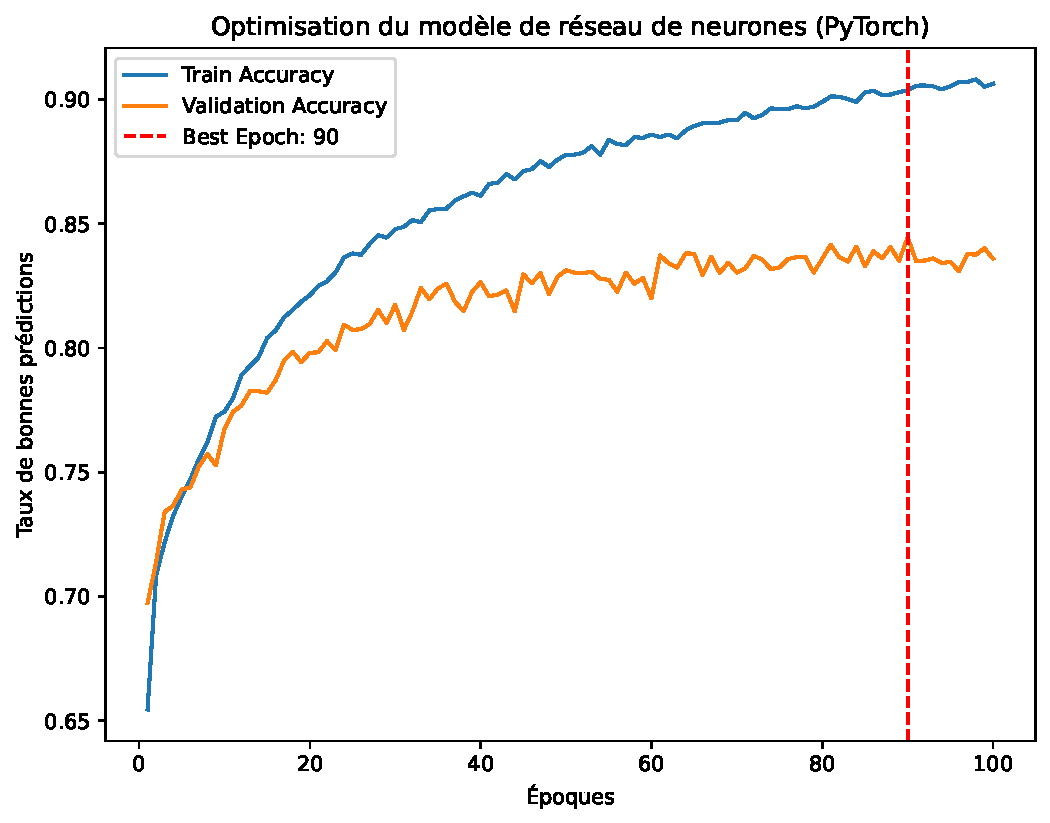
\includegraphics[keepaspectratio]{reseau_neurones_files/figure-pdf/cell-2-output-1.pdf}}

\begin{verbatim}

🔹 Meilleure époque : 90 avec une précision de validation de 84.45%

📊 Matrice de confusion :
[[1740  307    2    0    9    1   60]
 [ 340 2366   26    0   63   34    4]
 [   1   12 1268   22   13  114    0]
 [   0    0   16   88    0    6    0]
 [   7   68    7    0  295    3    0]
 [   2   21  104    4    4  559    0]
 [  45    6    0    0    0    0  770]]

📈 Taux de bien classés par classe :
Classe 1 : 82.11%
Classe 2 : 83.52%
Classe 3 : 88.67%
Classe 4 : 80.00%
Classe 5 : 77.63%
Classe 6 : 80.55%
Classe 7 : 93.79%

Taux de bien classés total : 84.49%
\end{verbatim}




\end{document}
